\documentclass[mode=present,style=simple,paper=screen]{powerdot}

\usepackage[utf8]{inputenc}
\usepackage[square]{natbib}
\usepackage{bibentry}
\usepackage{graphicx}
\usepackage{multirow}
\usepackage{bbding}
\usepackage{manfnt}
\usepackage{fourier}
\usepackage[labelfont=bf,textfont=sl,tableposition=top,scriptsize]{caption}
\usepackage{amsmath,amsfonts,amssymb,amsthm}
\usepackage{mathrsfs}

\theoremstyle{plain}% default
\newtheorem{thm}{Theorem}%[section]
\newtheorem{lem}{Lemma}
\newtheorem{prop} {Proposition}
\newtheorem{cor}{Corollary}
\theoremstyle{definition}
\newtheorem{defn}{Definition}%[section]
\newtheorem{conj}{Conjecture}%[section]
\newtheorem{exmp}{Example}%[section]
\theoremstyle{remark}
\newtheorem*{rem}{Remark}
\newtheorem{case}{Case}

\newcommand{\advice}[1]{\HandPencilLeft{} \emph{#1}}
\newcommand{\reminder}[1]{%
  \fcolorbox{blue}{white}{
    \begin{minipage}[l]{0.2\linewidth}
      \includegraphics[width=1\textwidth]{Figures/reminder}
    \end{minipage}
    \begin{minipage}[r]{0.8\linewidth}
      #1
    \end{minipage}
  }
}


\title{Statistical modelling of spatial extremes using the SpatialExtremes package}
\author{M. Ribatet}
\date{University of Montpellier}
% \date{
%   \begin{center}
%     $^\dag$ Laboratoire de Mathématiques et Application, Université de
%     Poitiers\\
%     $^\ddag$ Institut de Mathématiques et de Modélisation, Université
%     Montpellier 2
%   \end{center}
% }


\pdsetup{
  lf={The \texttt{SpatialExtremes} package},
  rf={Mathieu Ribatet},
  logohook=tr,
  logopos={.99\slidewidth,.99\slideheight},
  logocmd={},
  counters={thm,lem,prop,cor,defn,conj,exmp,case,figure},
}

\begin{document}

\maketitle

\begin{wideslide}[toc=]{Rationale for the \texttt{SpatialExtremes} package}
  \begin{quotation}
    ``The aim of the \texttt{SpatialExtremes} package is to provide
    tools for the areal modelling of extreme events. The modelling
    strategies heavily rely on the \textcolor{blue}{extreme value
      theory} and in particular \textcolor{blue}{block maxima}
    techniques---unless explicitly stated.''
  \end{quotation}

  As a consequence, most often
  \begin{itemize}
  \item the data used by the package \textcolor{blue}{have to be
      extreme}---do not pass daily values for instance;
  \item \textcolor{blue}{the marginal distribution family is fixed},
    i.e., the generalized extreme value distribution family, but you
    have hands on how within this family parameters change in space;
  \item \textcolor{blue}{the process family is fixed}, i.e.,
    max-stable processes, but you have hands on which type of
    max-stable processes to use.
  \end{itemize}
\end{wideslide}

\section[toc=0. Max-stable process]{0. About the inner structure of max-stable processes}

\begin{slide}{Spectral characterization}
  \vspace*{-1.75em}
  \onslide*{1}{
    \begin{equation*}
      Z(s) = \max_{i \geq 1} \zeta_i Y_i(s), \qquad s \in \mathcal{X},
    \end{equation*}
    where $\{\zeta_i\colon i \geq 1\}$ is a Poisson point process on
    $(0, \infty)$ with intensity measure $\mbox{d$\Lambda$}(\zeta) =
    \zeta^{-2} \mbox{d$\zeta$}$ and $Y_i$ independent copies of a
    (non-negative) stochastic process such that $\mathbb{E}\{Y(s)_+\}= 1$
    for all $s \in \mathcal{X}$.
  }%
  \onslide*{2-}{
    \begin{equation*}
      Z(s) = \max_{\varphi \in \Phi} \varphi(s), \qquad s \in \mathcal{X},
    \end{equation*}
    where $\Phi = \{\varphi_i\colon i \geq 1\}$ is a Poisson point
    process on $\mathbb{C}_0$ with an appropriate intensity measure.\vspace*{-0.5em}
    \begin{figure}
      \centering
      \includegraphics[width=0.95\textwidth]{Figures/IllustMaxStable}
    \end{figure}
  }
\end{slide}

\begin{wideslide}{Extremal functions}
  \vspace*{-2em}
  \begin{figure}
      \centering
      \onslide*{1}{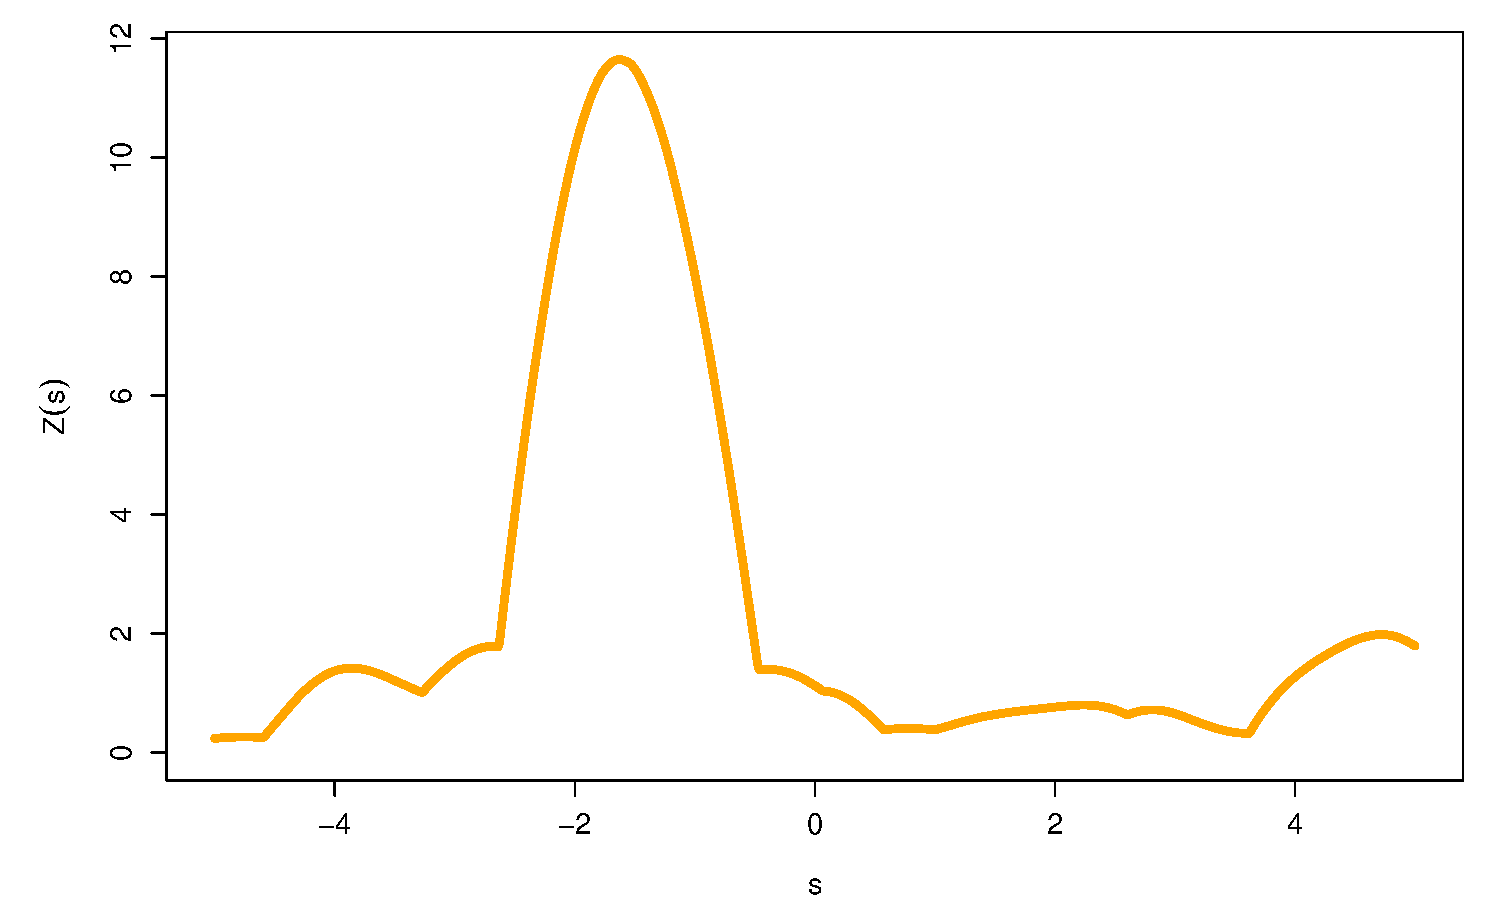
\includegraphics[width=0.7\textwidth]{Figures/IllustExtremalFct-1}}%
      \onslide*{2}{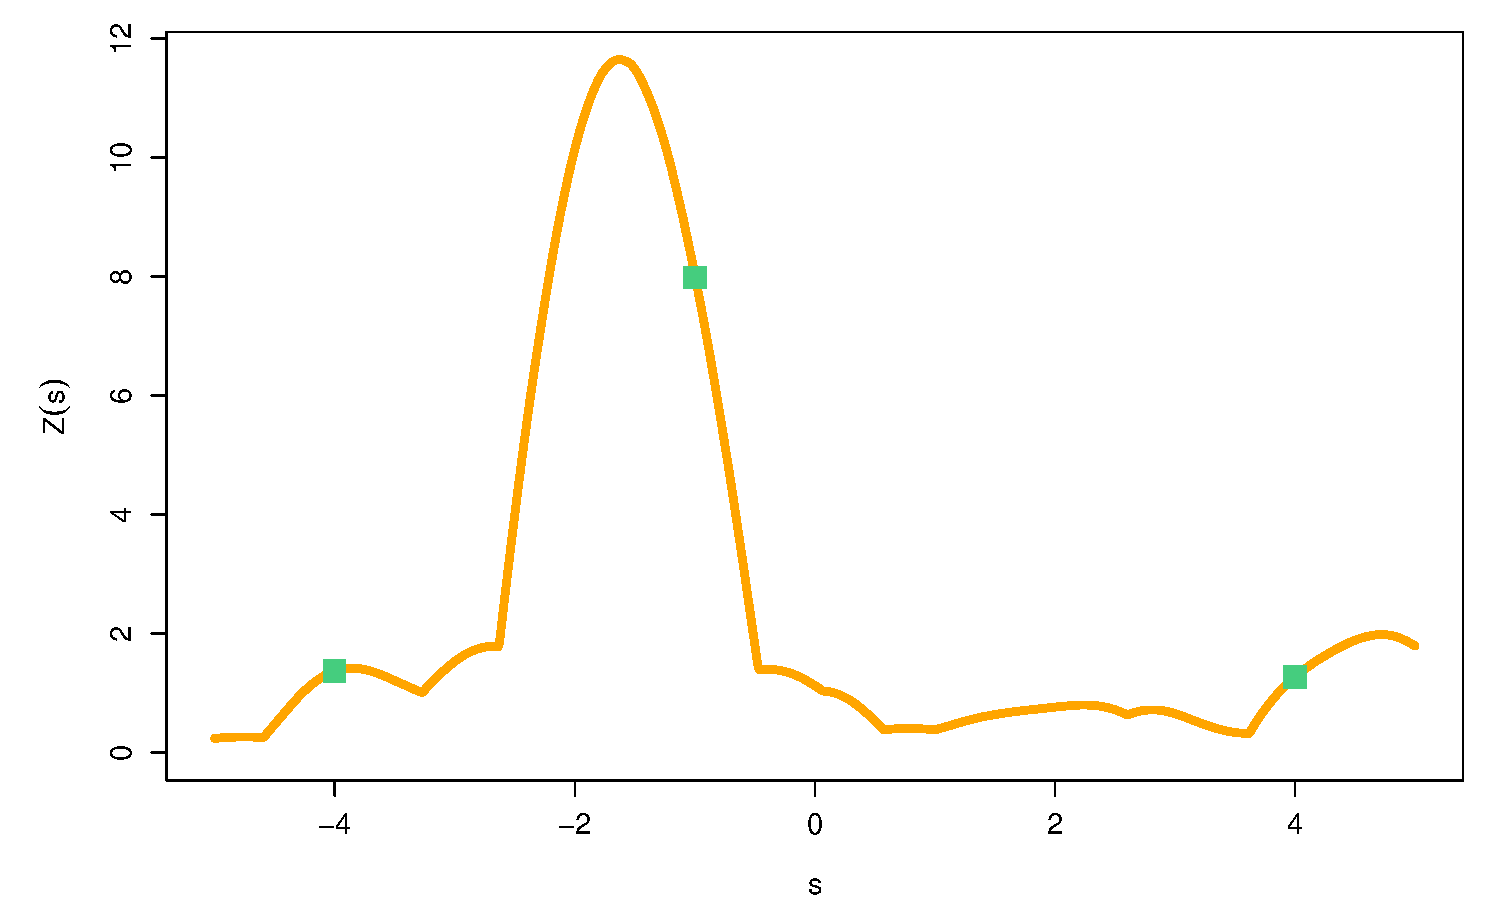
\includegraphics[width=0.7\textwidth]{Figures/IllustExtremalFct-2}}%
      \onslide*{3}{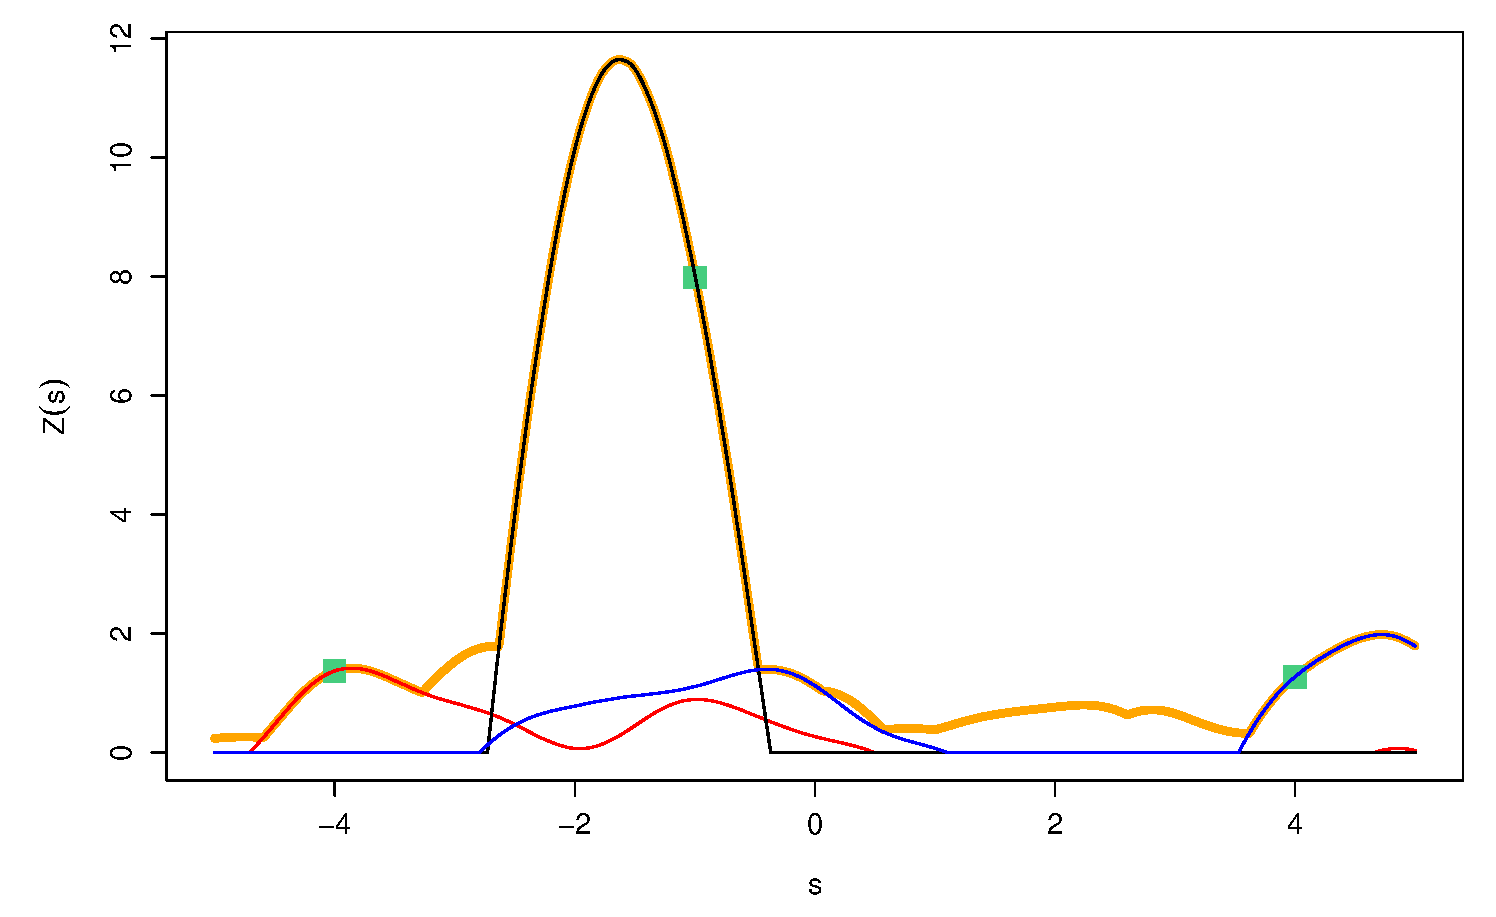
\includegraphics[width=0.7\textwidth]{Figures/IllustExtremalFct-3}}%
      \onslide*{4-}{\includegraphics[width=0.7\textwidth]{Figures/IllustExtremalFct-4}}%
    \end{figure}
    \vspace*{-2.75em}
    \begin{itemize}
    \item<3-> Hidden are the random functions
      $\Phi^+ = \{\varphi_1^+, \varphi_2^+, \ldots, \varphi_k^+\}$ of
      $\Phi$ such that
      \begin{equation*}
        \varphi_j^+(s_j) = Z(s_j), \qquad j = 1, \ldots, k, \qquad
        \text{\textcolor{red}{(extremal functions)}},
      \end{equation*}\vspace*{-1.5em}
    \item<4-> and the random functions $\varphi^- \in \Phi \setminus \Phi^+$,
      i.e., satisfying
      \begin{equation*}
        \varphi^-(s_j) < Z(s_j), \qquad j = 1, \ldots, k, \qquad
        \text{\textcolor{red}{(sub-extremal functions)}}
      \end{equation*}
    \end{itemize}
\end{wideslide}

\section{1. Data and descriptive analysis}

\begin{slide}[toc=Data format,method=direct]{Required data}
  Before introducing more advanced stuff, let's talk about data
  format. It is pretty simple: 
  \begin{description}
  \item[Observations] A numeric matrix such that \textcolor{blue}{each
      row is one realization of the spatial field}---or if you prefer
    one column per site;
  \item[Coordinates] A numeric matrix such that \textcolor{blue}{each
      row is the coordinates of one site}---or if you prefer the first
    column is for instance the longitude of all sites, the second one
    latitude, \ldots
  \end{description}
{\tiny
  \begin{minipage}[l]{.49\linewidth}
\begin{verbatim}
> data
       Valkenburg  Ijmuiden  De Kooy  ...
 1971         278        NA      360  ...
 1972         334        NA      376  ...
 1973         376        NA      365  ...
 1974         314        NA      304  ...
 1975         278        NA      278  ...
 1976         350        NA      345  ...
 1977         324        NA      298  ...
 1978         298        NA      329  ...
 1979         252        NA      298  ...
 ...
\end{verbatim}%
  \end{minipage}%
  \begin{minipage}[r]{.49\linewidth}
\begin{verbatim}
> coord
                        lon        lat
 Valkenburg           4.419     52.165
 Ijmuiden             4.575     52.463
 De Kooy              4.785     52.924
 Schiphol             4.774     52.301
 Vlieland             4.942     53.255
 Berkhout             4.979     52.644
 Hoorn                5.346     53.393
 De Bilt              5.177     52.101
 ...
\end{verbatim}
  \end{minipage}
}
\end{slide}

\begin{slide}[toc=,method=direct]{Additional covariates}
  In addition to the storage of observations and coordinates, you
  might want to use additional covariates. The latter can be of two
  types:
  \begin{description}
  \item[Spatial] A numeric matrix such that \textcolor{blue}{each
      column corresponds to one spatial covariate} such as elevation,
    urban/rural, \ldots
  \item[Temporal] A numeric matrix such that \textcolor{blue}{each
      column corresponds to one temporal covariate} such as time,
    annual mean temperature, \ldots
  \end{description}
{\tiny
  \begin{minipage}[l]{.49\linewidth}
\begin{verbatim}
> spat.cov
                     alt
 Valkenburg         -0.2
 Ijmuiden            4.4
 De Kooy             0.5
 Schiphol           -4.4
 Vlieland            0.9
 Berkhout           -2.5
 Hoorn               0.5
 De Bilt             2.0
 ...
\end{verbatim}
  \end{minipage}%
  \begin{minipage}[r]{.49\linewidth}
\begin{verbatim}
> temp.cov
               nao
 1971         1.87
 1972         1.57
 1973        -0.20
 1974        -0.95
 1975        -0.46
 1976         2.34
 1977        -0.49
 1978         0.70
 1979         1.11
 ...
\end{verbatim}
  \end{minipage}
}

\advice{It is always a good idea to name your columns and rows.}
\end{slide}

\begin{slide}[toc=First look]{Inspecting data}
  \begin{itemize}
  \item As usual, you should first \textcolor{blue}{scrutinize your
      data} (weird values, encoding of missing values, check out
    factors, \ldots). But you always do that, don't you?
  \item We focus on extremes, so you may wonder
    \begin{itemize}
    \item are my data \textcolor{blue}{extremes}, i.e., block maxima?
    \item is my \textcolor{blue}{block size} appropriate?
    \item what about \textcolor{blue}{seasonality}? Refine the block
      or use a temporal covariate?
    \end{itemize}
  \item You might want to \textcolor{blue}{check that the generalized
      extreme value family is sensible for your data}---the
    \texttt{evd} package + a few lines of code will do the job for you
    (homework) \ldots 
  \item This will generally be OK, but now you have to go a bit
    further by analyzing
    \begin{itemize}
    \item the spatial dependence;
    \item and the presence/absence of any spatial trends.
    \end{itemize}
  \end{itemize}
\end{slide}

\begin{slide}[toc=Spatial dependence]{Spatial dependence \citep{Cooley2006}}
  \begin{itemize}
  \item Essentially you want to check if your data exhibit any
    (spatial) dependence. If not why would you bother with spatial
    models?
  \item The most convenient way to do this is through the
    \textcolor{blue}{$F$-madogram} and its connection with the
    \textcolor{blue}{extremal coefficient}:
    \begin{equation*}
      \nu_F(h) = \frac{1}{2} \mathbb{E} [| F\{Z(o)\} - F\{Z(h)\}| ],
      \qquad \theta(h) = \frac{1 + 2 \nu_F(h)}{1 - 2 \nu_F(h)}.
    \end{equation*}
  \item The \texttt{fmadogram} function will estimate (empirically)
    the pairwise extremal coefficent from the $F$--madogram.
  \end{itemize}

  \reminder{\begin{equation*}
      \theta(h) = - z \log \Pr\{Z(s) \leq z, Z(s + h) \leq z\}
    \end{equation*}
    where $1 \leq \theta(h) \leq 2$, with complete dependence iff
    $\theta(h) = 1$ and independence iff $\theta(h) = 2$.}
\end{slide}

\begin{slide}[toc=]{Spatial dependence (2) \citep{Dombry2017}}
  \begin{itemize}
  \item Another recent summary measure of the spatial dependence is
    the \textcolor{blue}{extremal concurrence probability function}
    $p\colon h \mapsto p(h) \in [0, 1]$ where
    \begin{equation*}
      p(h) \onslide*{3-}{\textcolor{red}{:= p(s, s+h)}} = \Pr\{\exists! \varphi \in \Phi\colon \varphi(s) = Z(s), \
      \varphi(s+h) = Z(s+h)\},
    \end{equation*}
    \pause i.e., there is a single extremal function at position $s$ and
    $s+h$.
  \end{itemize}
  \vfill
  \reminder{%
    \begin{align*}
      p(h) &= \mathbb{E}[\mbox{sign}\{Z(s) - \tilde Z(s)\}
             \mbox{sign}\{Z(s+h) - \tilde Z(s+h)\}]\\
      &= \text{\textcolor{blue}{Kendall's $\tau$}},
    \end{align*}
    and $0 \leq p(h) \leq 1$ with complete dependence iff $p(h) =
    1$ and independence iff $p(h) = 0$.
  }
  \onslide{3-}{\textcolor{red}{\HandRight{} NB: here we assume a stationary dependence structure!}}
\end{slide}

\begin{wideslide}[toc=]{The \texttt{fmadogram} function}
  \vspace{-1.5em}
  \begin{itemize}
  \item Run the file \texttt{fmadogram.R}. You should get the figure
    below.
  \item<2-> You can also use a binned version with \texttt{n.bins =
      300}\ldots
  \end{itemize}
  \begin{figure}
    \centering
    \onslide*{1}{\includegraphics[width=.75\textwidth]{Figures/fmadogram}}
    \onslide*{2-}{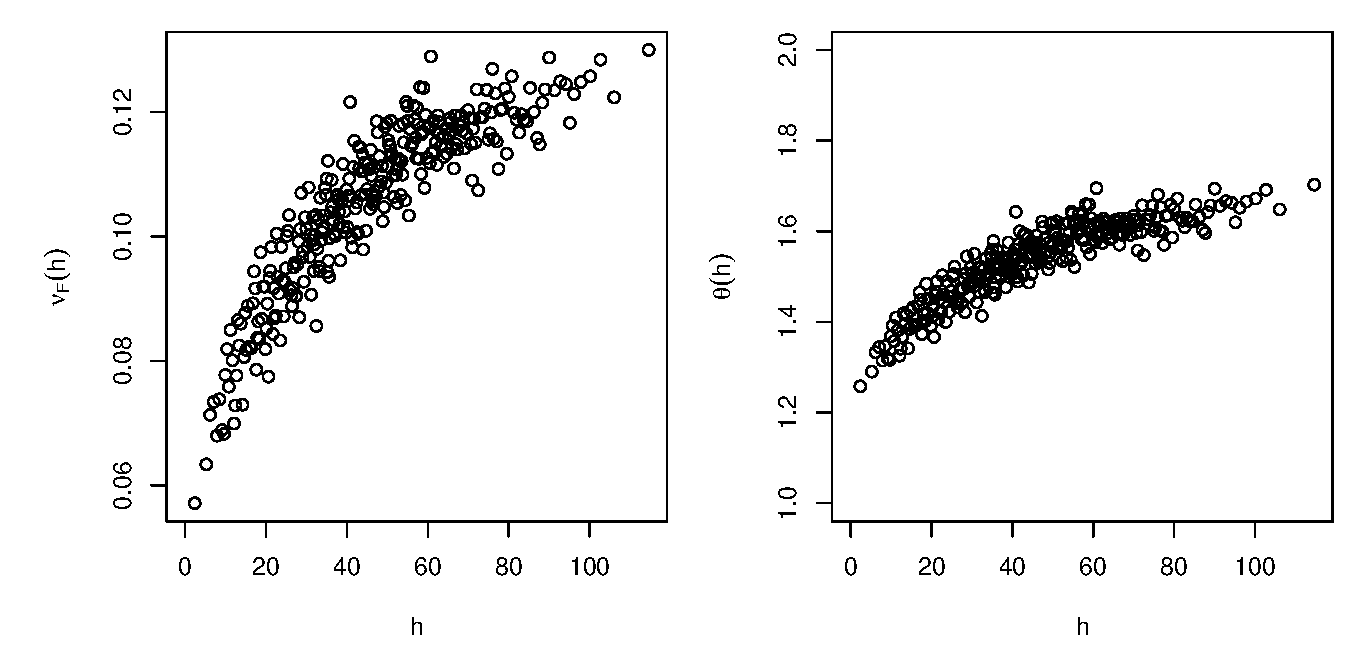
\includegraphics[width=.75\textwidth]{Figures/fmadogramBinned}}
    \caption{Use of the \texttt{fmadogram} function to assess the spatial dependence.}
    \label{fig:fmadogram}
  \end{figure}
  %%%\onslide{4}{\advice{Always think about what should be your spatial coordinates}}
\end{wideslide}

\begin{slide}[toc=]{The \texttt{concprob} function}
  \begin{itemize}
  \item Run the file \texttt{concprob.R}. You should get the figure
    below.
  \item<2-> You can also use a binned version with \texttt{n.bins =
      300}\ldots
  \end{itemize}
  \begin{figure}
    \centering
    \onslide*{1}{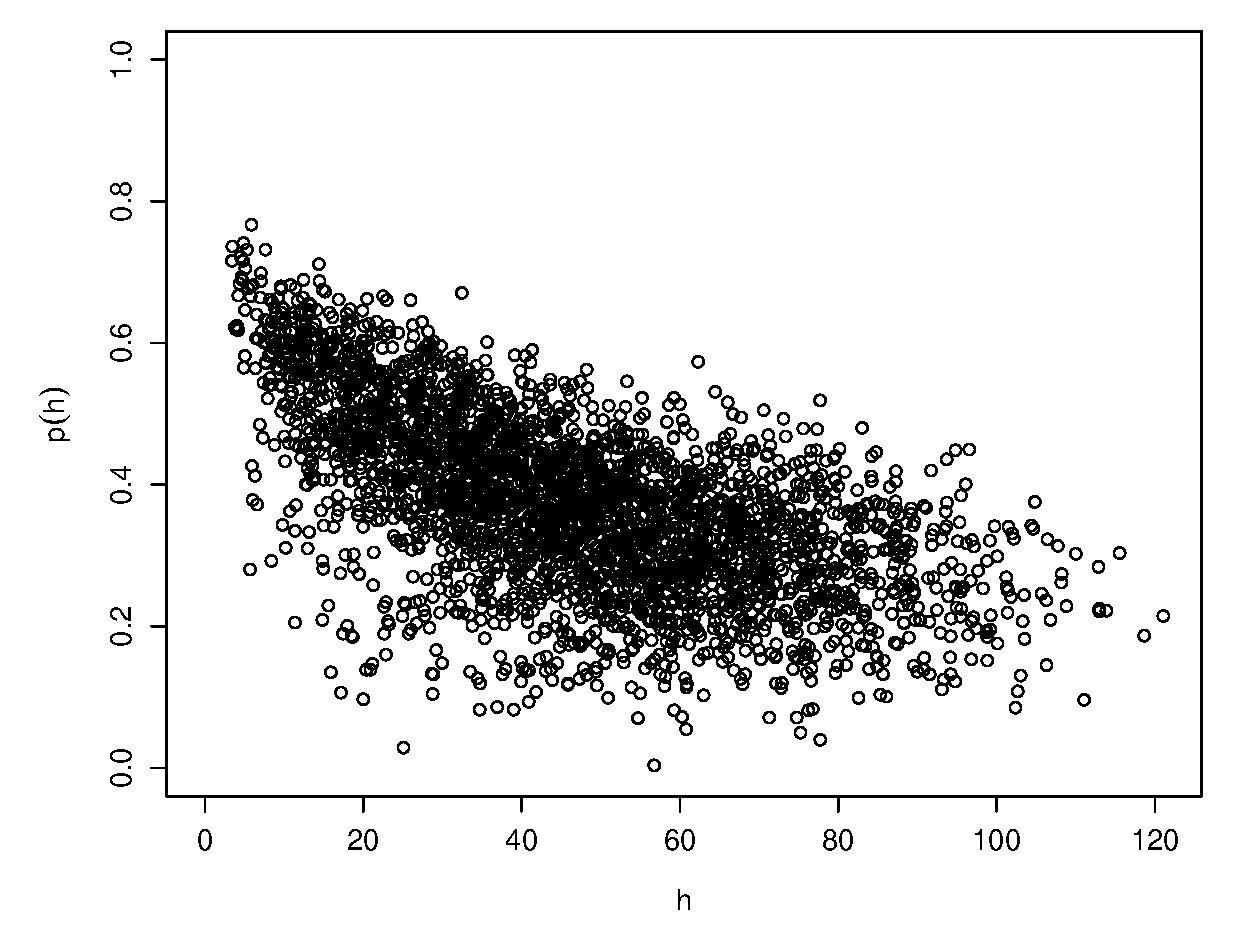
\includegraphics[width=.66\textwidth]{Figures/concprob}}
    \onslide*{2-}{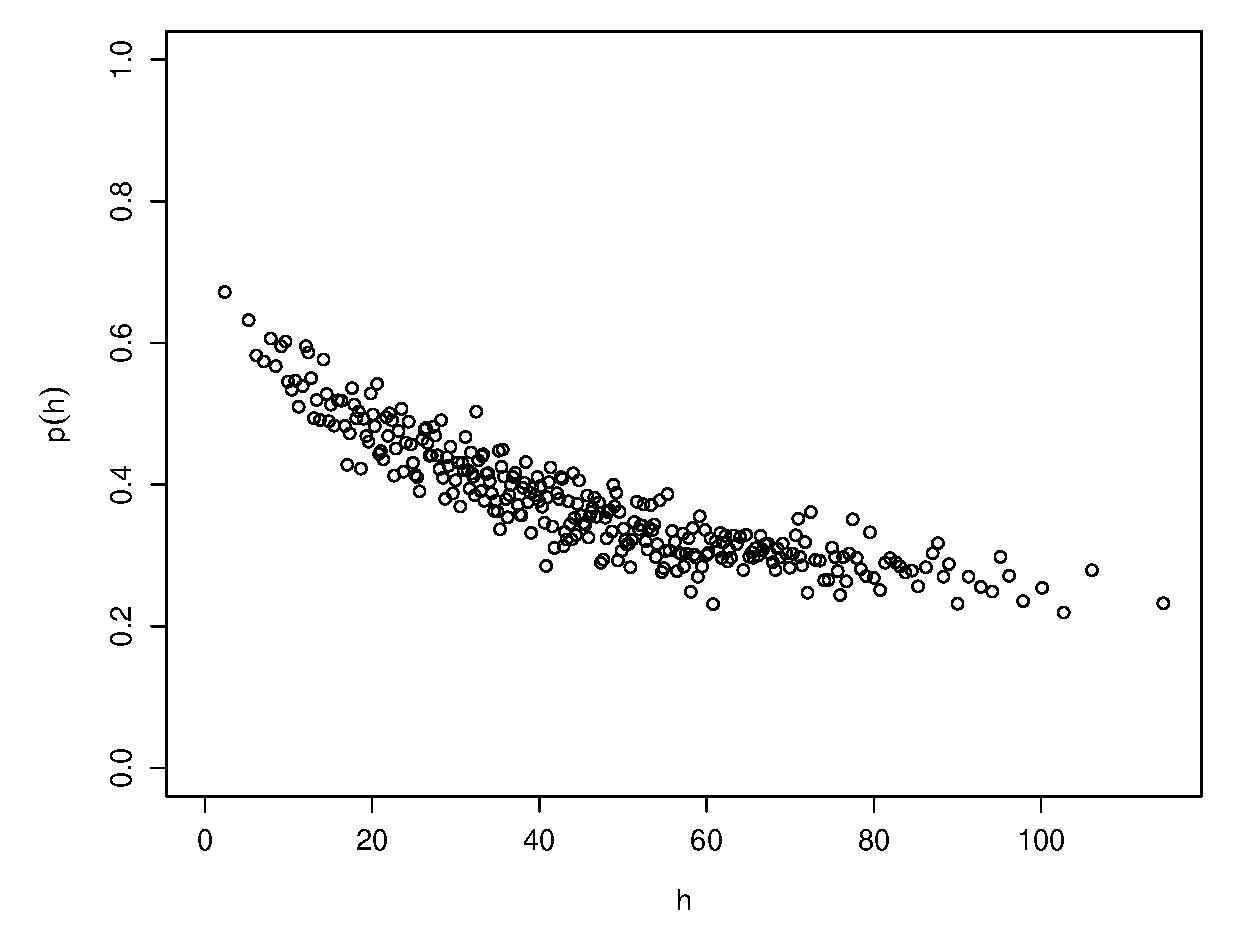
\includegraphics[width=.66\textwidth]{Figures/concprobBinned}}
    \caption{Use of the \texttt{concprob} function to assess the spatial dependence.}
  \end{figure}
  %%%\onslide{4}{\advice{Always think about what should be your spatial coordinates}}
\end{slide}

\begin{wideslide}[toc=]{As an aside (\texttt{AsAnAside.R}) \citep{Dombry2017}}
  \vspace*{-1.75em}
  \begin{itemize}
  \item We can estimate the spatial distribution of the extremal
    concurrence probability \textcolor{blue}{w.r.t. a given weather
      station}, e.g., plotting
    \begin{equation*}
      \left\{(s, p(\text{Zurich}, s))\colon s \in \mathcal{X}\right\},
    \end{equation*}\vspace*{-1.5em}
  \item<2-> or estimate the expected area of \textcolor{blue}{concurrence cells}
    \begin{equation*}
      A(s_0) =
      \mathbb{E}\left\{\int_\mathcal{X} 1_{\{\text{$s_0$ and $s$ are
            concurrent}\}} \mbox{d$s$} \right\} = \int_\mathcal{X}
        p(s_0, s) \mbox{d$s$}
    \end{equation*}
  \end{itemize}
  \vspace*{-1.5em}
  \begin{figure}
    \centering
    \includegraphics[width=0.45\textwidth]{Figures/concMap1}\hfill%
    \onslide{2}{\includegraphics[width=0.45\textwidth]{Figures/concMap2}}%
  \end{figure}
\end{wideslide}



\begin{wideslide}[toc=Spatial trends]{Spatial trends}
  %\vspace*{-1.5em}
  \begin{itemize}
  \item We can do a \textcolor{blue}{symbol plot} see the file \texttt{SpatialTrends.R}.
  \end{itemize}
  \pause
  \begin{figure}
    \centering
    \onslide*{2}{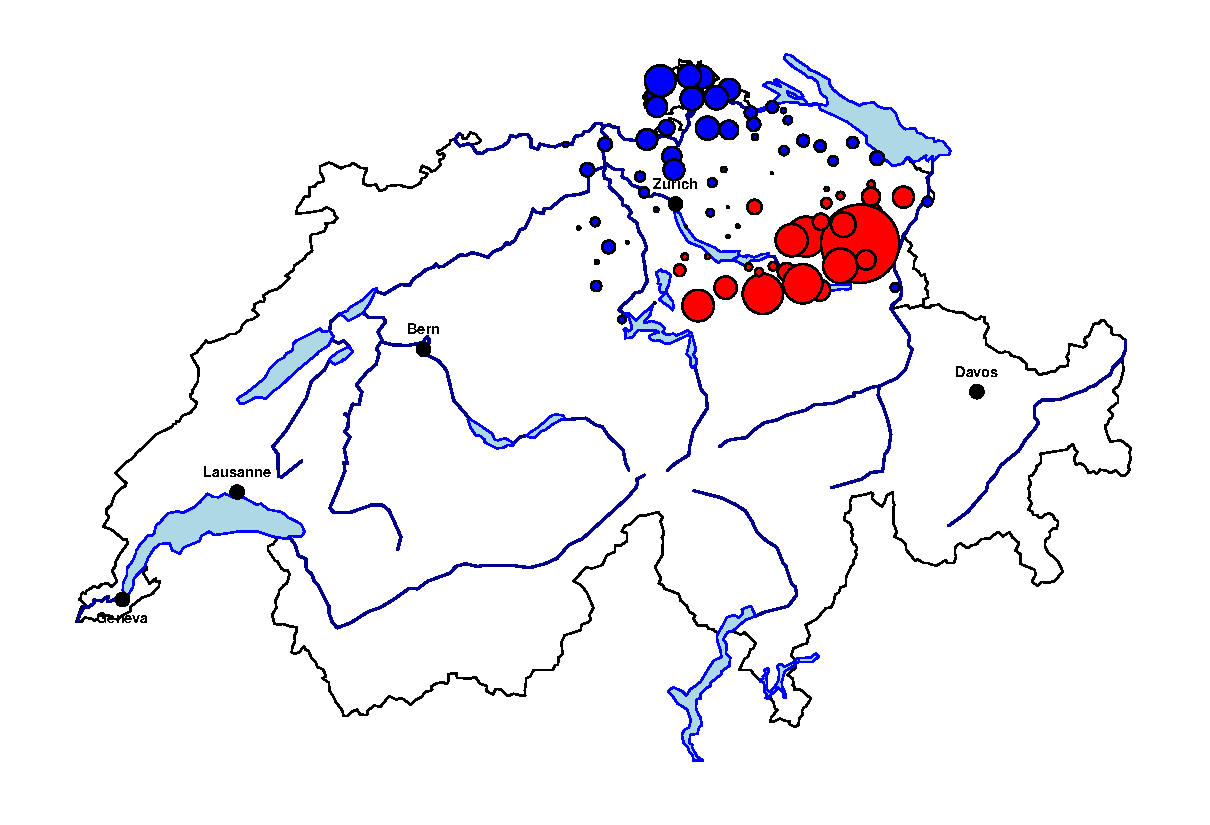
\includegraphics[width=0.5\textwidth]{Figures/symbolPlot}}
    \onslide*{3-}{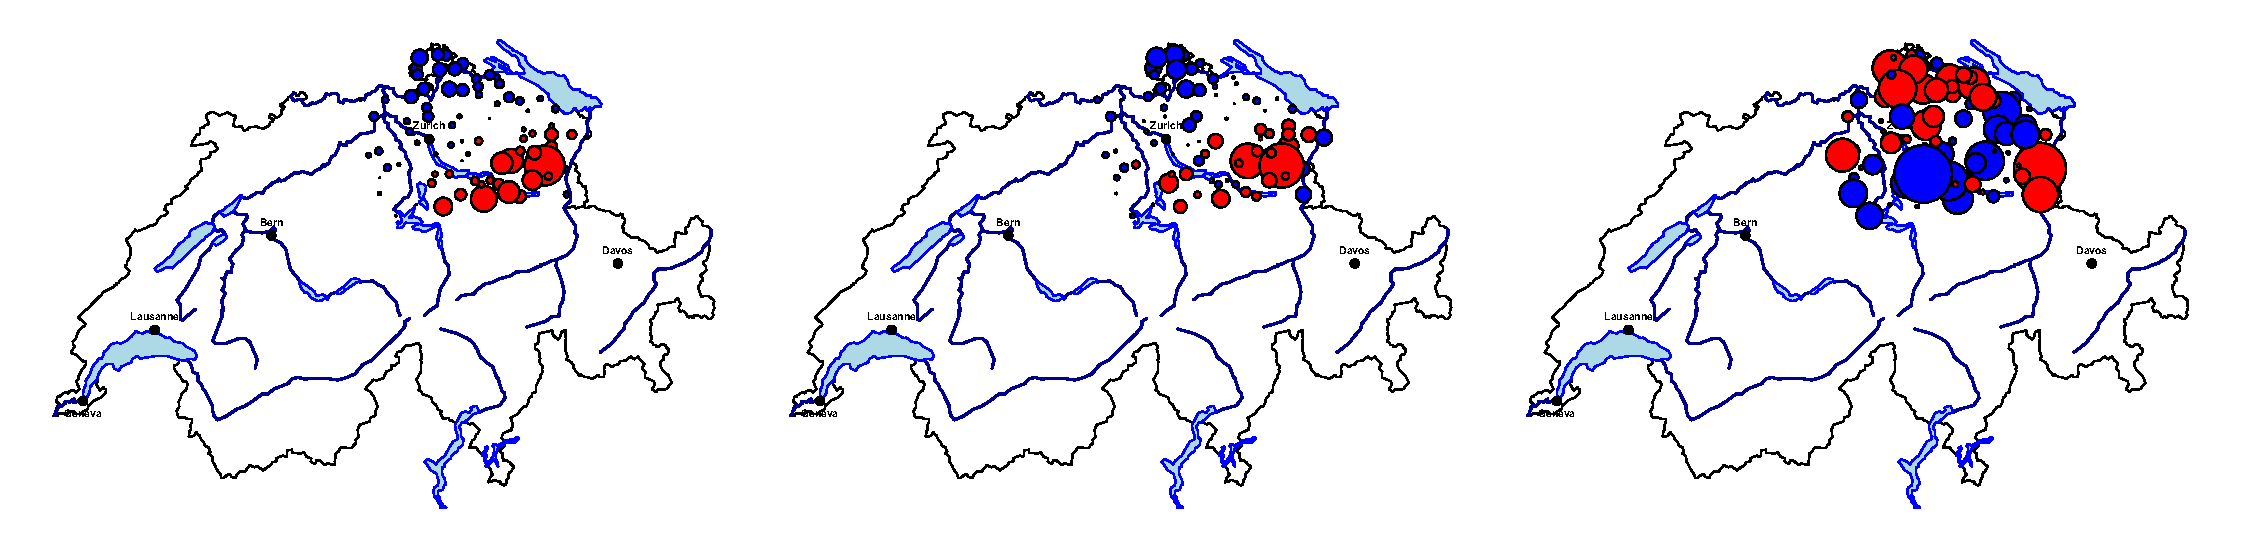
\includegraphics[width=\textwidth]{Figures/symbolPlot2}}
    \caption{Symbol plot for the Swiss precipitation data.}
  \end{figure}\vfill
  \onslide*{4-}{\advice{When exporting figures into eps/pdf, always
      pay attention to the aspect ratio.}}
\end{wideslide}

\begin{slide}[toc=Debrief \#1]{What we have learned so far (apart from
    using \texttt{SpatialExtremes})}
  \begin{itemize}
  \item The data exhibit some \textcolor{blue}{spatial
      dependence} and there is still some (weak) dependance at a
    separation lag of 100km.
  \item There's a clear \textcolor{blue}{north-west / south-east
      gradient} in the intensities of rainfall storms.
  \item In conclusion it makes sense to use max-stable
    \textcolor{blue}{processes} whose \textcolor{blue}{marginal
      parameters are not constant across space}.
  \item More specifically, we have:
    \begin{itemize}
    \item a clear north-west / south-east gradient for the location
      and scale parameters;
    \item no clear pattern for the shape parameter.
    \end{itemize}
  \end{itemize}
\end{slide}

\section{2. Simple max-stable processes}

\begin{slide}{Max-stable models}
  \begin{itemize}
  \item In this section we \textcolor{blue}{focus only on the spatial
      dependence} and so assume that the margins are known and
    \textcolor{blue}{unit Fréchet}---this is a standard choice in
    extreme value theory.
  \item From the spectral characterization
    \begin{equation*}
      Z(s) = \max_{i \geq 1} \zeta_i Y_i(s), \qquad s \in \mathcal{X},
    \end{equation*}
    we can propose several parametric models for spatial
    extremes. Hence by letting $Y$ to be
    \begin{description}
    \item[Gaussian densities] with random displacements we get the
      \textcolor{blue}{Smith} process;
    \item[Gaussian] we get the \textcolor{blue}{Schlather} process;
    \item[Log-normal] (with a drift) we get the \textcolor{blue}{Brown--Resnick} process;
    \item[Gaussian] but elevated to some power we get the
      \textcolor{blue}{Extremal-$t$} process.
    \end{description}
  \end{itemize}
\end{slide}

\begin{slide}[toc=]{Dependence parameters}
  \begin{description}
  \item[Smith] Elements of the covariance matrix appearing in the
    Gaussian densities;
  \item[Schlather] Parameters of the correlation function;
  \item[Brown--Resnick] Parameters of the semi-variogram;
  \item[Extremal--$t$] Parameters of the correlation function and
    degrees of freedom.
  \end{description}
  \begin{itemize}
  \item Since the margins are fixed, we only need to get estimates for
    the dependence parameters.
  \item How can we do that?
  \end{itemize}
\end{slide}

\begin{wideslide}[toc=Least squares,method=file]{Least squares
    (\texttt{leastSquares.R}) \citep{Smith1990}}
  \vspace*{-0.5em}
  \begin{equation*}
    \underset{\psi \in \Psi}{\arg \min} \sum_{1 \leq i < j \leq k}
    \left\{\theta(s_j - s_j; \psi) - \hat \theta(s_i - s_j)
    \right\}^2,
  \end{equation*}
  where $\theta(\cdot; \psi)$ is the extremal coefficient obtained
  from the max-stable model with dependence parameters set to $\psi$
  and $\hat \theta(\cdot)$ is any empirical estimates of the extremal
  coefficient, e.g., $F$--madogram based.

  \begin{minipage}[l]{.33\linewidth}
{\tiny
\begin{verbatim}
> M0
        Estimator: Least Squares
            Model: Schlather
         Weighted: TRUE
  Objective Value: 3592.429
Covariance Family: Whittle-Matern

Estimates
  Marginal Parameters:
  Assuming unit Frechet.

  Dependence Parameters:
  range   smooth
54.3239   0.4026

Optimization Information
  Convergence: successful
  Function Evaluations: 61
\end{verbatim}
}
  \end{minipage}
  \hfill
  \begin{minipage}[r]{.6\linewidth}
    \begin{figure}
      \centering
      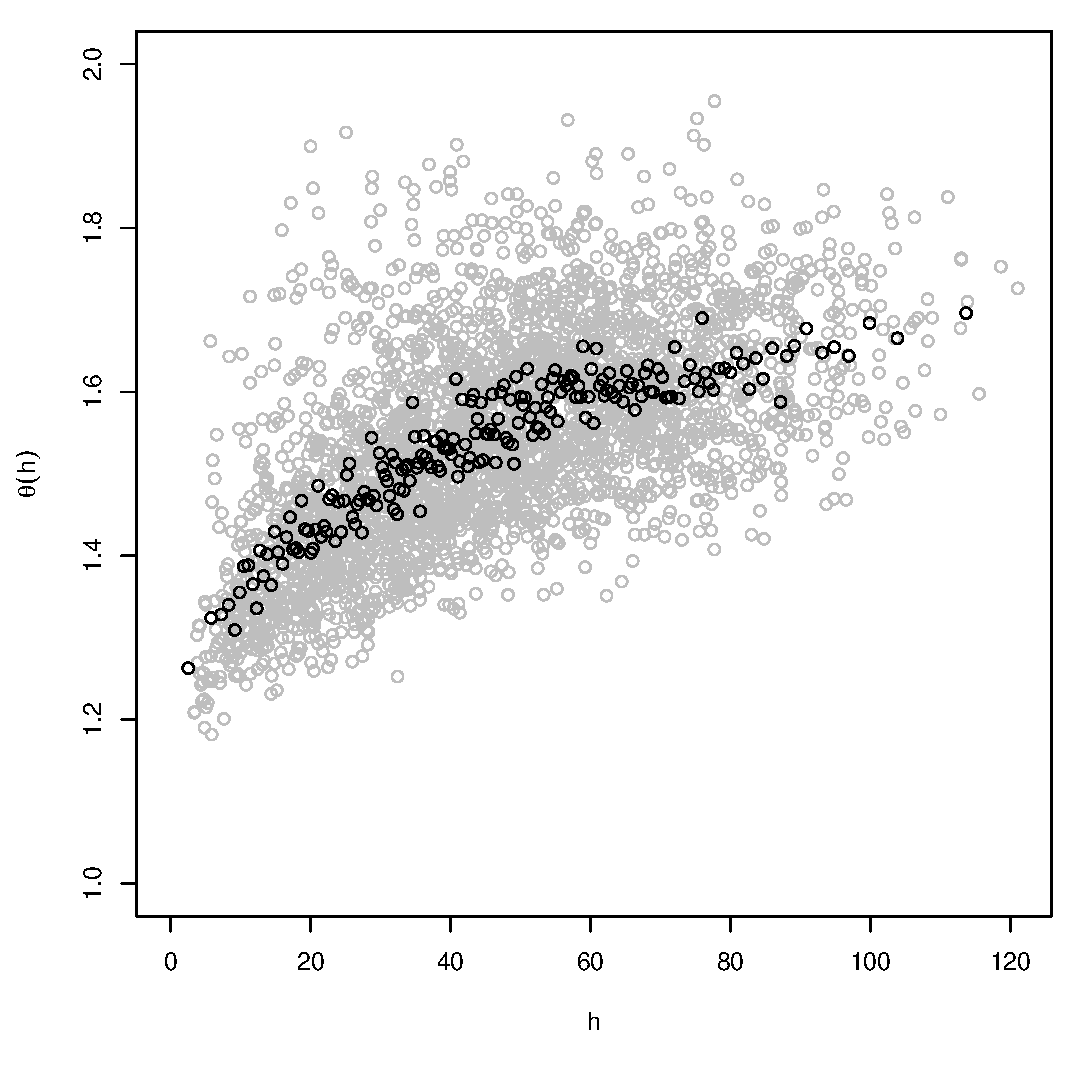
\includegraphics[width=0.49\textwidth]{Figures/empExtCoeffRain}%
      \onslide{2}{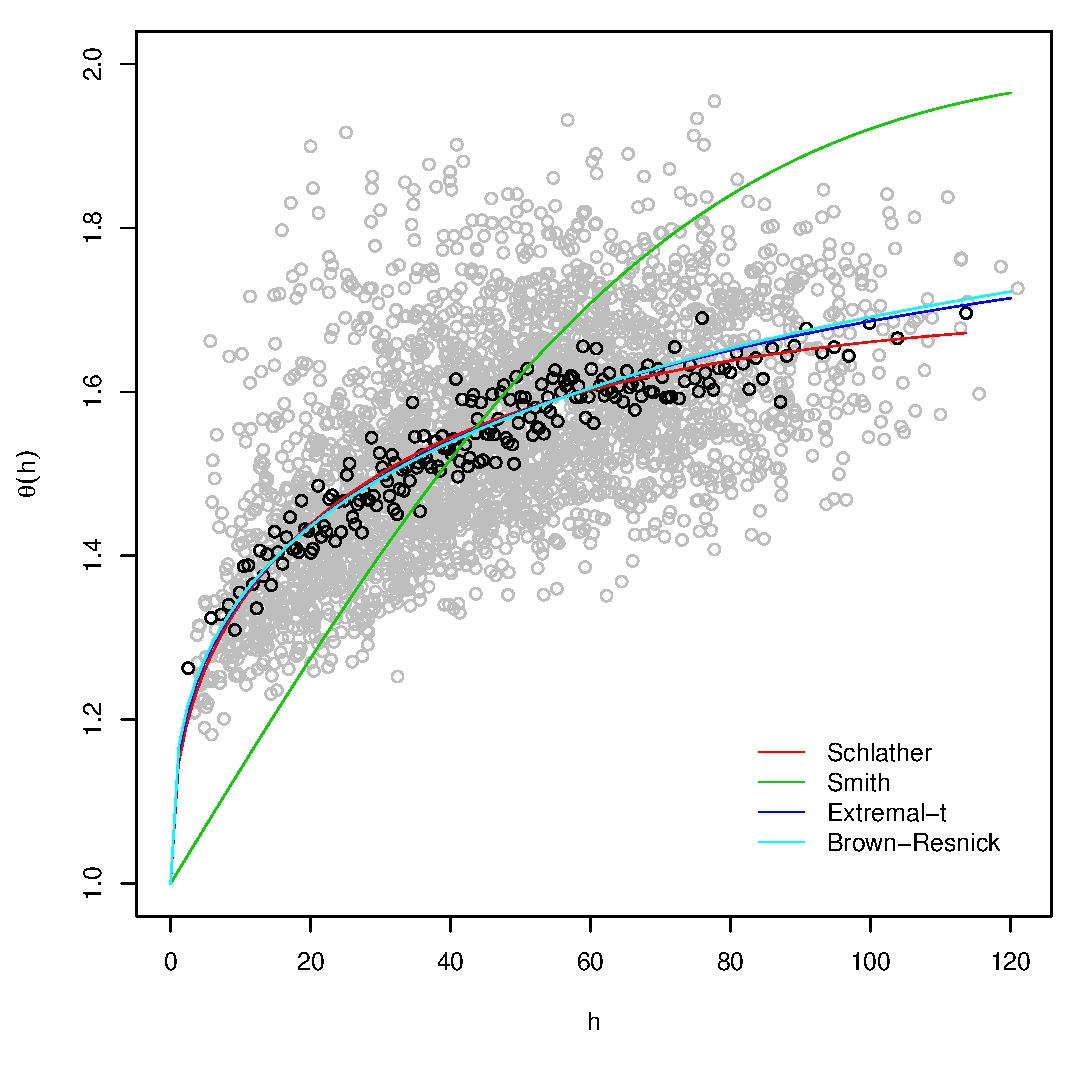
\includegraphics[width=0.49\textwidth]{Figures/leastSquares}}
      \caption{Fitting simple max-stable processes from least
        squares.}
      \label{fig:leastSquares}
    \end{figure}
  \end{minipage}
\end{wideslide}

\begin{wideslide}[toc=Pairwise likelihood,method=file]{Pairwise
    likelihood (\texttt{pairwiseLlik.R}) \citep{Padoan2010}}
  \vspace*{-2em}
  \begin{equation*}
    \underset{\psi \in \Psi}{\arg \max} \sum_{\ell = 1}^n \sum_{1 \leq
      i < j \leq k} \log f\{z_\ell(s_i), z_\ell(s_j); \psi\},
  \end{equation*}
  where $f(\cdot, \cdot; \psi)$ is the bivariate density of the
  considered max-stable model.

    \begin{minipage}[l]{.33\linewidth}
      {\tiny
\begin{verbatim}
        Estimator: MPLE
            Model: Schlather
         Weighted: FALSE
   Pair. Deviance: 1136863
              TIC: 1137456
Covariance Family: Whittle-Matern

Estimates
  Marginal Parameters:
  Assuming unit Frechet.

  Dependence Parameters:
  range   smooth
50.1976   0.3713

Standard Errors
  range   smooth
20.7085   0.0789

Asymptotic Variance Covariance
        range       smooth
range   428.841018   -1.570081
smooth   -1.570081    0.006225
Optimization Information
  Convergence: successful
  Function Evaluations: 67
\end{verbatim}
}
  \end{minipage}
  \hfill
  \begin{minipage}[r]{.6\linewidth}
    \begin{figure}
      \centering
      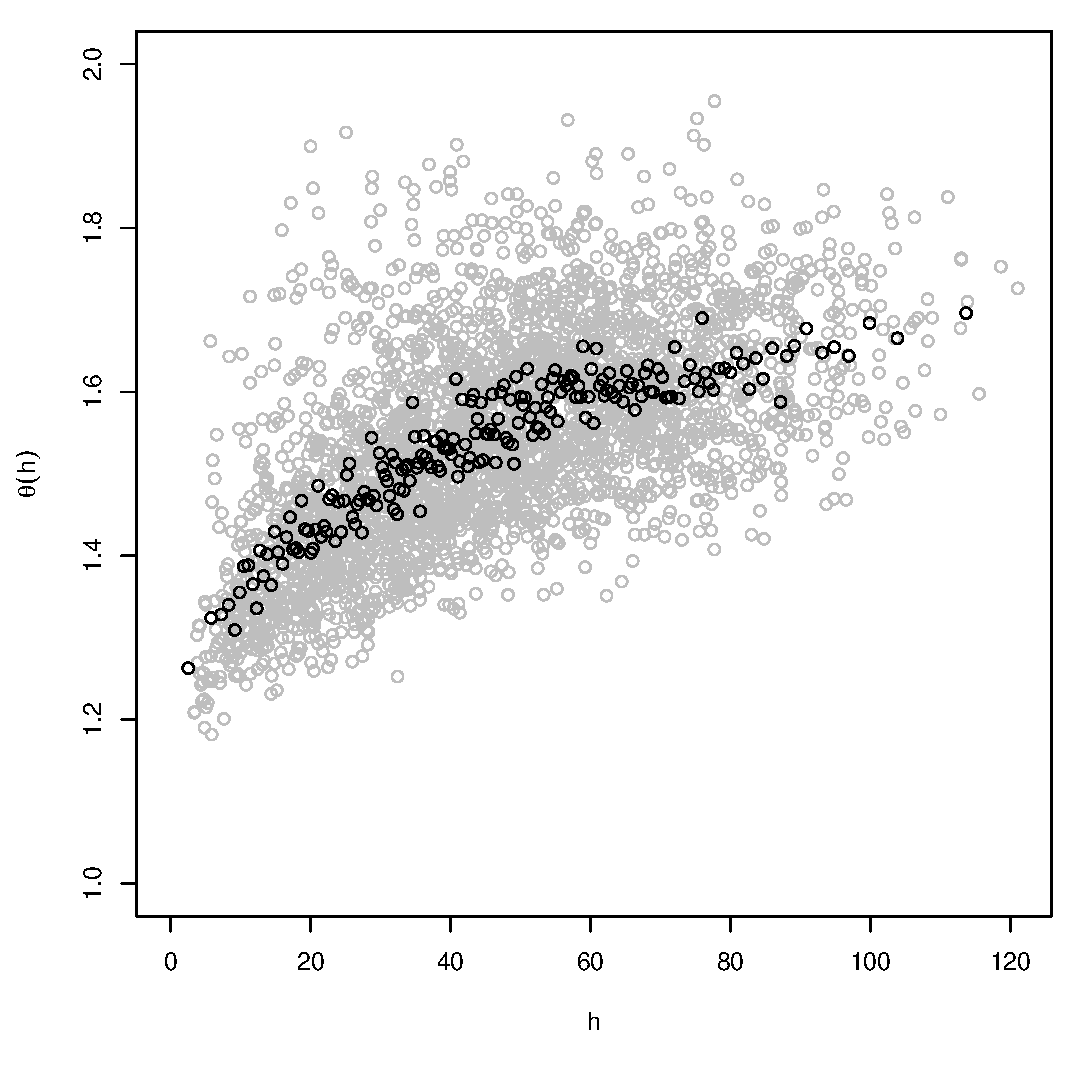
\includegraphics[width=0.49\textwidth]{Figures/empExtCoeffRain}%
      \onslide{2}{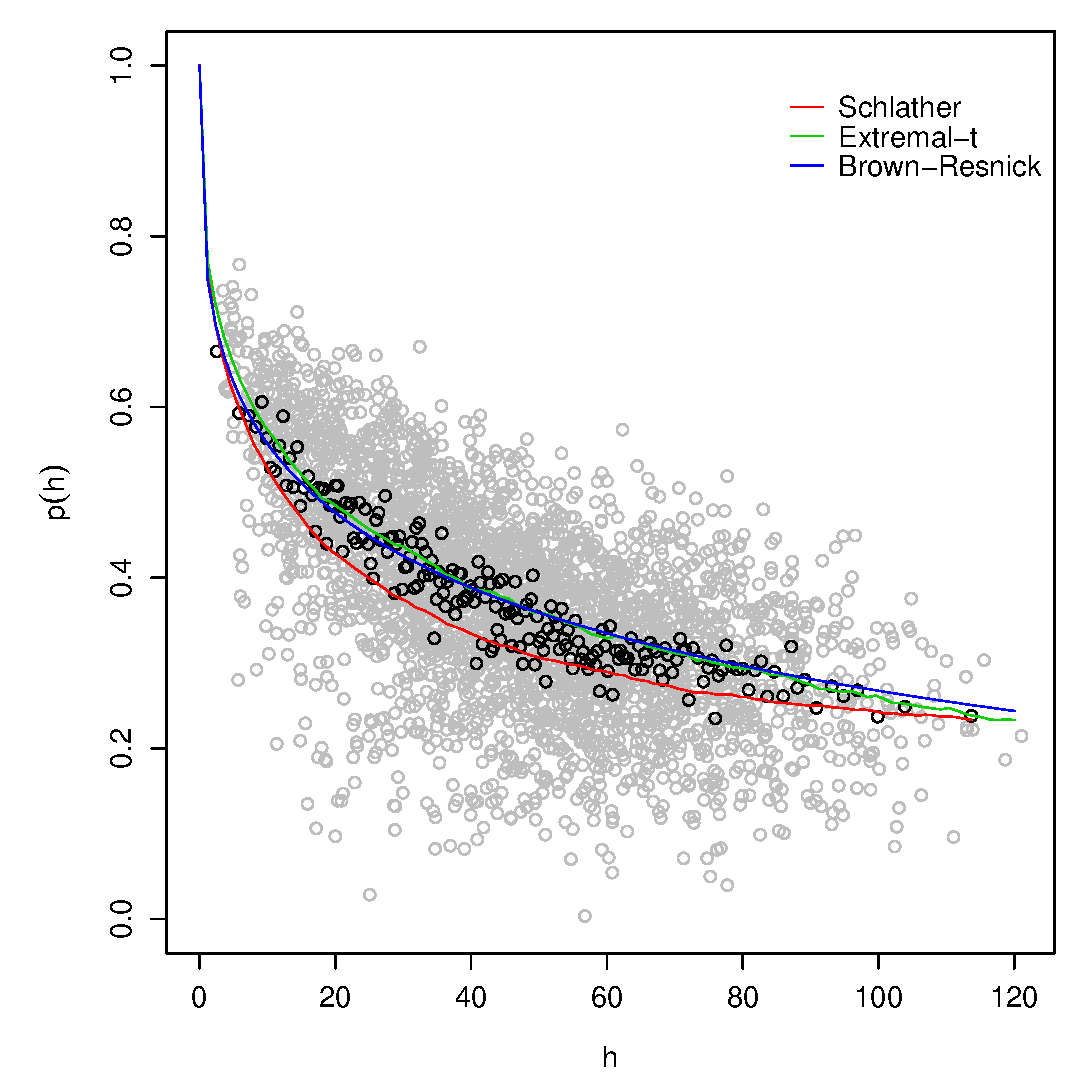
\includegraphics[width=0.49\textwidth]{Figures/pairwiseLlik}}
      \caption{Fitting simple max-stable processes maximizing pairwise
        likelihood.}
      \label{fig:pairLlik}
    \end{figure}
  \end{minipage}
\end{wideslide}

\begin{slide}[method=direct,toc= Model selection]{Model Selection \citep{Varin2005}}
  \begin{itemize}
  \item The advantage of the pairwise likelihood estimator over the
    least squares one is that you can do \textcolor{blue}{model
      selection}.
  \item For instance one can use the ${\rm TIC}$,
    \textcolor{blue}{Takeuchi Information Criterion} or sometimes
    known as ${\rm CLIC}$, Composite Likelihood Information Criterion,
    \begin{equation*}
      {\rm TIC} = 2 \ell_{\rm pairwise}(\hat \psi) - 2
      \mbox{tr}\{J(\hat \psi) H^{-1} (\hat \psi)\},
    \end{equation*}
    $H(\hat\psi) = \mathbb{E} \{\nabla^2 \ell_{\rm pairwise}(Y; \hat
    \psi) \}$, $J(\hat \psi) = \mbox{Var}\{\nabla \ell_{\rm
      pairwise}(Y; \hat\psi)\}$.
  \item From our previous fitted models, we get
{\tiny
\begin{verbatim}
> TIC(M0,M1,M2)
     M1      M2      M0
1133660 1134823 1137449
\end{verbatim}
}
  \end{itemize}
\end{slide}

\begin{slide}[toc=Simulation,method=direct]{Simulating simple max-stable processes
    (\texttt{simulation.R}) \citep{Schlather2002,Dombry2016}}
  \begin{itemize}
  \item Once you have fitted a suitable model, you usually want to
    simulate from it.
  \item Simulation from max-stable models is rather complex, recall
    that
    \begin{equation*}
      Z(s) = \max_{i \geq 1} \zeta_i Y_i(s), \qquad s \in \mathcal{X}.
    \end{equation*}
  \end{itemize}
  \begin{minipage}[l]{.6\linewidth}
{\tiny
\begin{verbatim}
sim <- rmaxstab(n.obs, cbind(x, y), "twhitmat", DoF = 4,
+               nugget = 0, range = 3, smooth = 1)
> sim
            [,1]       [,2]      [,3]      [,4]       [,5]
 [1,]  3.8048914  0.4767980 6.3613989 1.4548317  1.0433912
 [2,]  1.2200332  0.6711422 0.8078701 2.0928629  0.7537061
 [3,]  0.5466466  2.0498561 4.8852572 2.3497976  0.6857268
 [4,]  ...
\end{verbatim}
}
  \end{minipage}
  \hfill
  \begin{minipage}[r]{.33\linewidth}
    \begin{figure}
      \centering
      \includegraphics[width=\textwidth]{Figures/simulation}
      \caption{One simulation on a 50 x 50 grid from the extremal--$t$
        model. (log scale)}
    \end{figure}
  \end{minipage}
\end{slide}

\begin{slide}[toc=Debrief \#2]{What we have learned so far (apart from
    using \texttt{SpatialExtremes})}
  \begin{itemize}
  \item The Smith model is clearly not a sensible model for our
    data---because of its linear behaviour near the origin;
  \item Schlather, Brown--Resnick and Extremal--$t$ seems relevant;
  \item According to the ${\rm TIC}$, the Extremal--$t$ should be
    preferred.
  \end{itemize}
\end{slide}

\section{3. Trends surfaces}

\begin{slide}[toc=]{From generalized extreme value margins to unit
    Fréchet ones}
  \begin{itemize}
  \item Alright! We are able to handle the spatial dependence, but
    \textcolor{blue}{we assume that our data have unit Fréchet
      margins}. This is not realistic at all!
  \item Fortunately, if $Y \sim {\rm GEV}(\mu, \sigma, \xi)$ then
    \begin{equation*}
      Z = \left(1 + \xi \frac{Y - \mu}{\sigma} \right)^{1 / \xi} \sim
      \text{Unit Fréchet}=\mbox{GEV}(1,1,1).
    \end{equation*}
    \pause
  \item And since we are extreme value and spatial guys
    \begin{equation*}
      Z\textcolor{blue}{(s)} = \left\{1 + \xi\textcolor{blue}{(s)}
        \frac{Y\textcolor{blue}{(s)} -
          \mu\textcolor{blue}{(s)}}{\sigma\textcolor{blue}{(s)}}
      \right\}^{1 / \xi\textcolor{blue}{(s)}}, \qquad s \in \mathcal{X},
    \end{equation*}
    is a simple max-stable process.
  \item Hence we can use the maximum pairwise likelihood estimator as
    before---up to an \textcolor{blue}{additional Jacobian term}.
  \end{itemize}
\end{slide}

\begin{slide}[toc=Spatial GEV]{Omitting the spatial dependence}
  \begin{itemize}
  \item With simple max-stable models, we omitted the marginal parameters.
  \item Here we will \textcolor{blue}{omit the spatial dependence for
      a while} and consider locations as being
    \textcolor{blue}{mutually independent}, i.e., use independence
    likelihood
    \begin{equation*}
      \underset{\psi \in \Psi}{\arg \max} \sum_{i=1}^k \ell_{\rm
        GEV}\{y(s_i); \psi\}.
    \end{equation*}
  \item This is a kind of ``\emph{spatial GEV}'' where $\psi$ is a
    vector of marginal parameters.
  \end{itemize}
\end{slide}

\begin{slide}[toc=,method=direct]{Defining trend surfaces}
  \vspace*{-1em}
  \begin{figure}
    \centering
    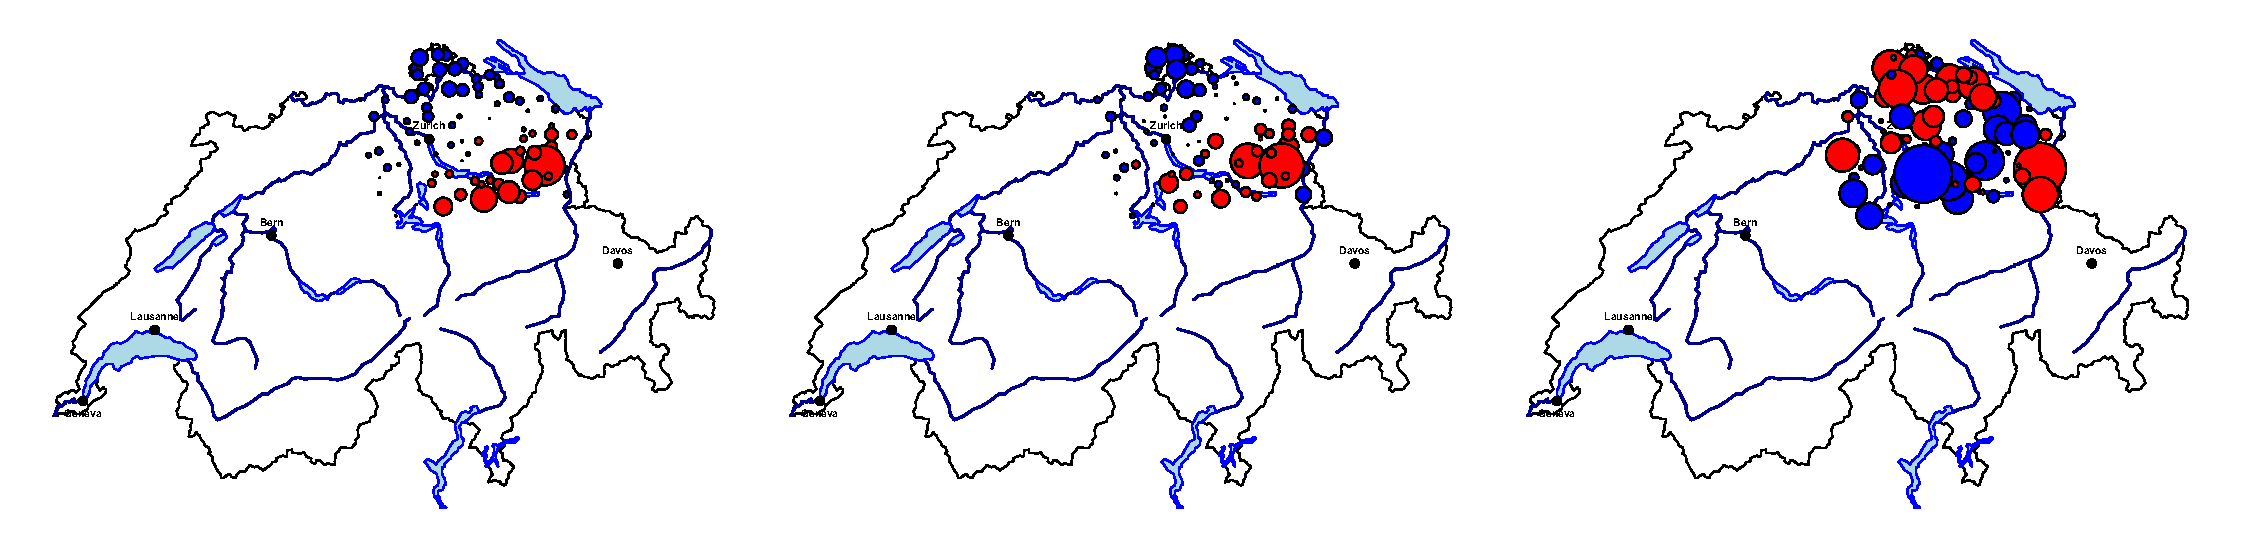
\includegraphics[width=\textwidth]{Figures/symbolPlot2}
    \caption{Symbol plot for the Swiss precipitation data.}
  \end{figure}
  This suggests that
  \begin{align*}
    \mu(s) &= \beta_{0,\mu} + \beta_{1, \mu} {\rm lon}(s) + \beta_{2,
      \mu} {\rm lat}(x) + \beta_{3, \mu} {\rm lon}(s) \times {\rm lat}(s),\\
    \sigma(s) &= \beta_{0,\sigma} + \beta_{1, \sigma} {\rm lon}(s) + \beta_{2,
      \sigma} {\rm lat}(s) + \beta_{3, \sigma} {\rm lon}(s) \times {\rm lat}(s),\\
    \xi(s) &= \beta_{0,\xi},
  \end{align*}
  or equivalently with the \texttt{R} language\vspace*{-0.5em}
{\small
\begin{verbatim}
loc.form <- scale.form <- y ~ lon * lat; shape.form <- y ~ 1
\end{verbatim}
}
\end{slide}

\begin{slide}[toc=,method=direct]{Fitting the \emph{spatial GEV} model
    (\texttt{spatialGEV.R}) \citep{Davison2012}}
  \vspace*{-1em}
  \tiny{
\begin{verbatim}
      Model: Spatial GEV model
   Deviance: 29303.81
        TIC: 29499.38

    Location Parameters:
locCoeff1  locCoeff2  locCoeff3  locCoeff4
   27.132      1.846     -3.656     -1.080
       Scale Parameters:
scaleCoeff1  scaleCoeff2  scaleCoeff3  scaleCoeff4
     9.7850       0.7023      -1.0858      -0.5531
       Shape Parameters:
shapeCoeff1
     0.1572

Standard Errors
  locCoeff1    locCoeff2    locCoeff3    locCoeff4  scaleCoeff1  scaleCoeff2
    1.13326      0.34864      0.45216      0.38361      0.76484      0.28446
scaleCoeff3  scaleCoeff4  shapeCoeff1
    0.31267      0.27566      0.05878

Asymptotic Variance Covariance
             locCoeff1   locCoeff2   locCoeff3   locCoeff4   scaleCoeff1
locCoeff1     1.2842711   0.1131400  -0.1740921  -0.0729564   0.6570988
locCoeff2     0.1131400   0.1215498  -0.0623759   0.0149596   0.0521630
locCoeff3    -0.1740921  -0.0623759   0.2044448   0.0576622  -0.1086629
locCoeff4    -0.0729564   0.0149596   0.0576622   0.1471593  -0.0346376
scaleCoeff1   0.6570988   0.0521630  -0.1086629  -0.0346376   0.5849729
...

Optimization Information
  Convergence: successful
  Function Evaluations: 2135
\end{verbatim}
    }
\end{slide}

\begin{wideslide}[toc=Prediction \#1]{Get predictions (\texttt{predictionSpatialGEV.R})}
  \begin{figure}
    \centering
    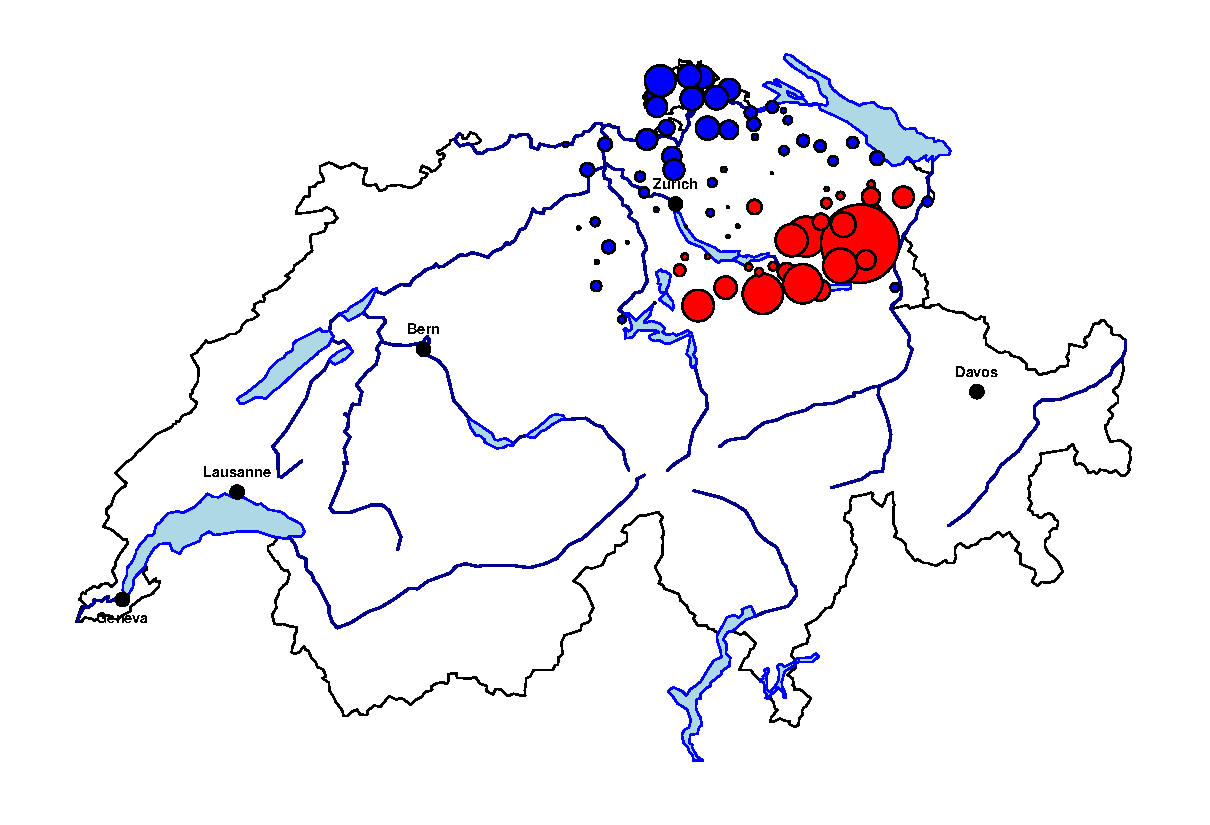
\includegraphics[width=0.5\textwidth]{Figures/symbolPlot}%
    \includegraphics[width=.5\textwidth]{Figures/predictionSpatialGEV}
    \caption{Left: symbol plot. Right: Prediction of the pointwise
      25-year return levels from a fitted spatial GEV model.}
    \label{fig:prediction}
  \end{figure}
  \pause
  \begin{itemize}
  \item But don't we forget something??? \pause
  \item Model selection?
  \end{itemize}
\end{wideslide}

\begin{slide}[toc=Model selection \#2,method=direct]{Model selection \#2
    (\texttt{modelSelection.R}) \citep{Chandler2007,Kent1982}}
  \begin{itemize}
  \item Typically here we would like to test if a given covariate is
    required or not
  \item Hence we're dealing with nested model for which
    \textcolor{blue}{composite likelihood ratio test} are especially
    suited
    \begin{equation*}
      2 \{\ell_{\rm composite}(\hat \psi) - \ell_{\rm composite}(\hat
      \phi_{\lambda_0}, \lambda_0)\} \longrightarrow \sum_{j=1}^p
      \lambda_j X_i, \qquad n \to \infty.
    \end{equation*}
  \end{itemize}
{\tiny
\begin{verbatim}
Eigenvalue(s): 2.7 1.95

Analysis of Variance Table
   MDf Deviance Df  Chisq Pr(> sum lambda Chisq)
M2   7    29328
M0   9    29306  2 22.265               0.008273 **
---
Signif. codes:  0 ‘***’ 0.001 ‘**’ 0.01 ‘*’ 0.05 ‘.’ 0.1 ‘ ’ 1
\end{verbatim}
}
\advice{Always check that your models are nested. The code won't do
  that for you!}
\end{slide}

\begin{slide}[toc=Debrief \#3]{What we have learned so far (apart from
    using \texttt{SpatialExtremes})}
  \begin{itemize}
  \item Based on the \texttt{spatial GEV} model, we identify what
    seems to be relevant trend surfaces for the marginal parameters:
    \begin{align*}
      \mu(s) &= \beta_{0,\mu} + \beta_{1, \mu} {\rm lon}(s) + \beta_{2,
        \mu} {\rm lat}(s) + \beta_{3,\mu} {\rm lon}(s) {\rm lat(s)},\\
      \sigma(s) &= \beta_{0,\sigma} + \beta_{1, \sigma} {\rm lon}(s) + \beta_{2,
        \sigma} {\rm lat}(s),\\
      \xi(s) &= \beta_{0,\xi},
    \end{align*}
  \end{itemize}
\end{slide}

\section{4. General max-stable processes}

\begin{wideslide}[toc=Fitting,method=direct]{Fitting a max-stable process with trend
    surfaces}
  \begin{itemize}
  \item Now it's time to combine everything, i.e.,
    \textcolor{blue}{trend surfaces + dependence}.
  \item The syntax won't be a big surprise
  \end{itemize}
  {\tiny
\begin{verbatim}
M0 <- fitmaxstab(rain, coord[,1:2], "twhitmat", nugget = 0, loc.form, scale.form, shape.form)

       Estimator: MPLE
            Model: Extremal-t
         Weighted: FALSE
   Pair. Deviance: 2237562
              TIC: 2249206
Covariance Family: Whittle-Matern

Estimates
  Marginal Parameters:
    Location Parameters:
locCoeff1  locCoeff2  locCoeff3  locCoeff4
27.136295   0.060145  -0.164755  -0.001117
       Scale Parameters:
scaleCoeff1  scaleCoeff2  scaleCoeff3
    9.88857      0.02869     -0.04581
       Shape Parameters:
shapeCoeff1
     0.1727
  Dependence Parameters:
   range    smooth       DoF
225.9452    0.3645    4.1566
...
\end{verbatim}
}
\end{wideslide}

\begin{wideslide}[method=direct]{Model checking \citep{Davison2012}}
  \begin{minipage}[l]{.49\linewidth}
    \begin{itemize}
    \item When you want to check your fitted max-stable model, you
      usually want to check if
      \begin{itemize}
      \item observations at each single location are well modelled:
        \textcolor{blue}{return level plot};
      \item the dependence is well captured: \textcolor{blue}{extremal
          coefficient function}.
      \end{itemize}
    \item This can be done using a single line of code
\begin{verbatim}
> plot(M0)
\end{verbatim}
    \end{itemize}
  \end{minipage}
  \hfill
  \onslide{2}{
  \begin{minipage}[r]{.49\linewidth}
    \begin{figure}
      \centering
      \includegraphics[width=\textwidth]{Figures/checkFinalModel}
      \caption{Model checking for a fitted max-stable process having
        trend surfaces.}
    \end{figure}
  \end{minipage}
}
\end{wideslide}

\begin{wideslide}{Predictions (\texttt{simulationFinal.R})}
  \begin{itemize}
  \item Prediction works as for the \emph{spatial GEV model} thanks to
    the \texttt{predict} function.
  \item But beware these predictions are pointwise---no spatial
    dependence at all!!!
  \item If you want to do take into account spatial dependence then
    you need to simulate from your fitted model.
  \end{itemize}
  \vspace*{-2em}
  \begin{figure}
    \centering
    \includegraphics[width=0.5\textwidth]{Figures/oneSimFinalModel}
    \caption{One simulation from our fitted extremal--$t$ model with trend surfaces.}
  \end{figure}
\end{wideslide}

\section{5. Conclusion}

\begin{wideslide}[toc=]{What we haven't seen}
  \begin{itemize}
  \item Using weighted pairwise likelihood;
  \item Many (many!) utility functions. Highly recommended to have a
    look at the documentation;
  \item The package has a vignette: \texttt{vignette("SpatialExtremesGuide")};
  \item Copula models---although I do not recommend their use for
    spatial extremes;
  \item Bayesian hierarchical models;
  \item Unconditional simulations: several implementations (including
    exact simulations)
  \item Conditional simulations---really CPU demanding.
  \end{itemize}
  \pause
  \HandRight{} A rather recent review on max-stable processes with R
  code is given by \citet{Ribatet2013b}
  \vfill
  \begin{center}
    \Large THANK YOU!
  \end{center}
  \vfill
\end{wideslide}

\begin{wideslide}{References}
  \vspace*{-1.5em}
  {\footnotesize
  \bibliographystyle{apalike}
  \nobibliography{/Users/Mathieu/Dropbox/biblio_ribatet}

  \begin{itemize}
  \item[\checkmark] \bibentry{Chandler2007}
  \item[\checkmark] \bibentry{Cooley2006}
  \item[\checkmark] \bibentry{Davison2012}
  \item[\checkmark] \bibentry{Dombry2016}
  \item[\checkmark] \bibentry{Dombry2017}
  \item[\checkmark] \bibentry{Padoan2010}
  \item[\checkmark] \bibentry{Ribatet2013b}
  \item[\checkmark] \bibentry{Schlather2002}
  \item[\checkmark] \bibentry{Smith1990}
  \item[\checkmark] \bibentry{Varin2005}
  \end{itemize}
  }
\end{wideslide}

%\bibliography{/Users/Mathieu/Dropbox/biblio_ribatet}
%\bibliographystyle{apalike}


\end{document}

%%% Local Variables:
%%% mode: latex
%%% TeX-master: t
%%% End:
